%!TEX root = ../TTK4900-MHT.tex

\chapter{Tracking runtime plot}

\begin{figure}[H]
\centering
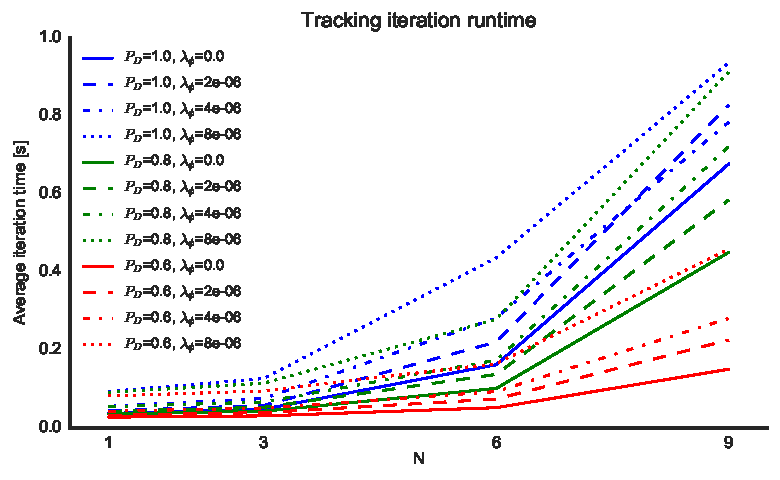
\includegraphics{Figures/plots/Scenario0_Tracking-Runtime.pdf}
\caption{Scenario 0 --- Tracking runtime}\label{fig:scenario0_tracking_runtime}
\end{figure}

\begin{figure}
\centering
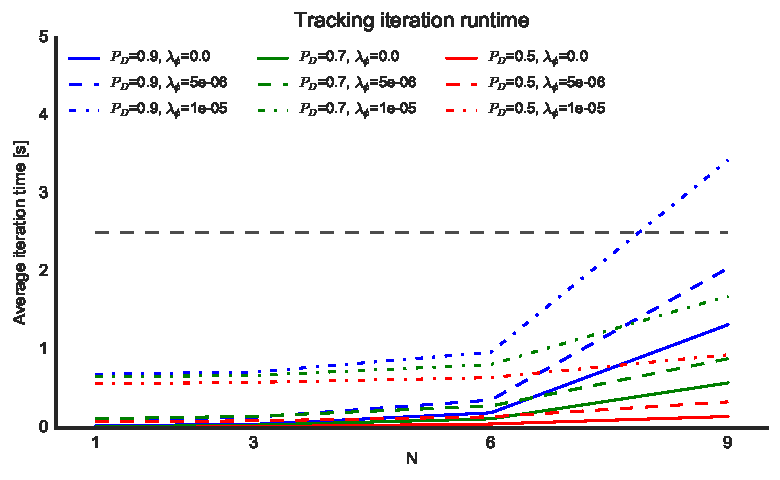
\includegraphics{Figures/plots/Scenario1_Tracking-Runtime.pdf}
\caption{Scenario 1 --- Tracking runtime}\label{fig:scenario1_tracking_runtime}

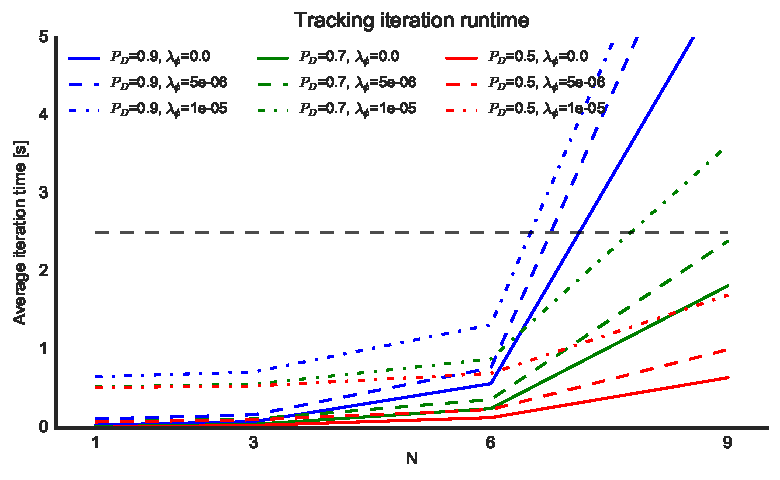
\includegraphics{Figures/plots/Scenario2_Tracking-Runtime.pdf}
\caption{Scenario 2 --- Tracking runtime}\label{fig:scenario2_tracking_runtime}
\end{figure}

\begin{figure}
\centering
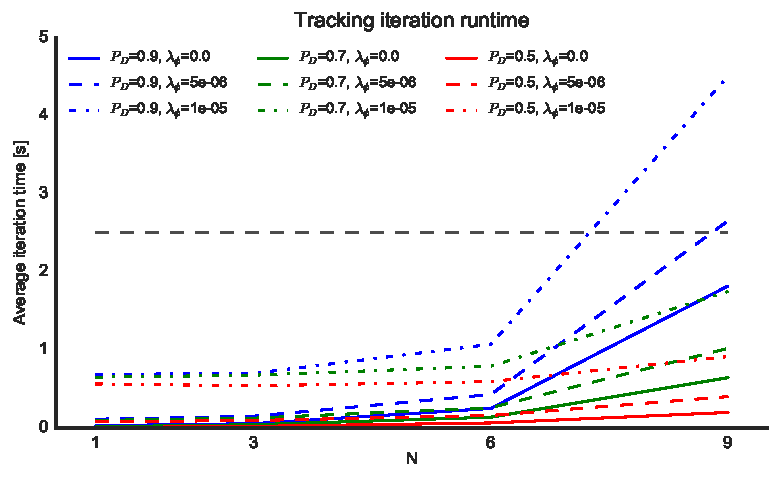
\includegraphics{Figures/plots/Scenario3_Tracking-Runtime.pdf}
\caption{Scenario 3 --- Tracking runtime}\label{fig:scenario3_tracking_runtime}

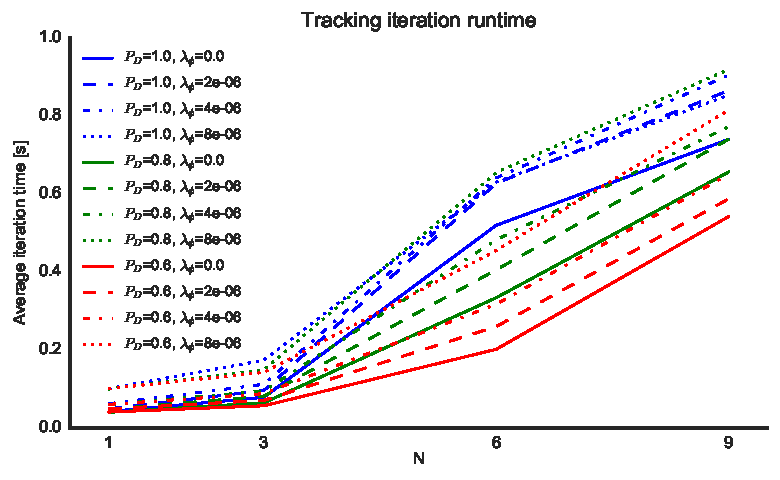
\includegraphics{Figures/plots/Scenario4_Tracking-Runtime.pdf}
\caption{Scenario 4 --- Tracking runtime}\label{fig:scenario4_tracking_runtime}
\end{figure}
